\documentclass{beamer}

\usepackage[utf8]{inputenc}
\usepackage[TS1,T1]{fontenc}
\usepackage[ngerman]{babel}
\usepackage{graphicx}

\usenavigationsymbolstemplate{}

\setbeamertemplate{footline}{%
\begin{beamercolorbox}[wd=\paperwidth,ht=2.25ex,dp=1ex]{date in head/foot}%
\hspace*{1ex} 
\insertframenumber{} / \inserttotalframenumber
\end{beamercolorbox}
}%


\newcommand{\sectionframe}[1]
{
\section{#1}
\begin{frame}
    \vspace{1cm}
    \begin{center}
        \begin{LARGE}
            #1
        \end{LARGE}
    \end{center}
\end{frame}
}

\title{\bf Model-View-Controller}
\author{SE3 Team}
\date{Juni 2009}

\begin{document}

\frame{\titlepage}

\frame{\vspace{1cm}\tableofcontents}

\sectionframe{Model-View-Controller}

%% the main definitions for the report (KOMA-Script based)
\documentclass[11pt,a4paper]{scrreprt}
\usepackage[T1]{fontenc}
\usepackage[utf8]{inputenc}
\usepackage[german,english]{babel}
\usepackage{layouts}

%% include the parameters for the text layout

\begin{document}
\selectlanguage{\german}
\title{MVC - Paradigma}
\author{Silvio Kunaschk}
\date{\today}
\maketitle
\tableofcontents
%% include the title and chapter files

MVC - Yooo geht los jetzt!

\pagediagram

\end{document}


\sectionframe{Analyse}

%% the main definitions for the report (KOMA-Script based)
\documentclass[11pt,a4paper]{scrreprt}
\usepackage[T1]{fontenc}
\usepackage[utf8]{inputenc}
\usepackage[german,english]{babel}
\usepackage{graphicx}

\begin{document}
\selectlanguage{\german}
\title{{\Huge \bf MVC}\\[0.55em]{\LARGE WeatherInfo - Analysedokument}}
\author{{\bf SE3 Team}\\Uwe Hausbrand}
\date{Juni 2009}

\maketitle

\tableofcontents

\chapter{Anforderungen an das Programm}

Als Beispielapplikation haben wir uns ein Wetterdatenprogramm \"uberlegt, wobei die
Wetterdaten f\"ur mehrere Tage und unterschiedlich St\"adte in verschiedenen Arten
angezeigt und in mindestens einer auch ver\"andert werde k\"onnen.

\section{Analyse der Anforderungen}

\subsection{Das Model}
In unserem Model ist eine tabellen\"ahnliche Struktur f\"ur die Datenspeicherung und
Datenverwaltung sinnvoll, da wir als Spalten die einzelnen Tage des zu beobachtenden
Zeitraums und als Zeilen die einzelnen St\"adte benutzen k\"onnen. Als einen ausreichenden
Zeitraum erachten wir f\"unf Tage, da die Wahrscheinlichkeit f\"ur eine
korrekte Wettervorhersage f\"ur einen l\"angeren Zeitraum sehr gering ist.
Als Datenquelle k\"onnen wir zum einen einen Online-Wetterdienst benutzen oder, f\"ur Testzwecke,
statische Daten. Dazu sollte das Programm beim Start seinen Datenbestand aus der Onlinequelle
aktualisieren.

Folgende Daten sollen vom Model zur Verf\"ugung gestellt werden:
\begin{itemize}
  \item Temperatur
  \item Windst\"arke
  \item Windrichtung
  \item Bew\"olkung
  \item Koordinaten (Latitude und Longitude)
\end{itemize}

\subsection{Die Views}
Folgende Views sollen beispielhaft implementiert werden:
\begin{itemize}
  \item Eine tabellarische Ansicht aller St\"adte f\"ur alle Tage und die Anzeige von
  Temperatur und Bew\"olkung f\"ur die einzelnen St\"adte. In dieser View soll eine
  \"Anderung des Temperatureintrages f\"ur einen beliebigen Tag und einer beliebigen
  Stadt m\"oglich sein. Ebenso soll der Nutzer die angezeigten St\"adte \"uber einen Filter
  einschr\"anken k\"onnen. Die \"Anderung der Temperatur soll direkt im Tabellenfeld erfolgen,
  die Filterdefinition in einer Textbox im unteren Viewbereich. Als Filter soll eine
  Namenseinschr\"ankung der St\"adte dienen.

  \item Eine Tagesansicht einer einzelnen Stadt mit allen zur Verf\"ugung stehenden
  Daten. Dabei sollte die Stadt und der angezeigte Tag \"uber eine Auswahlbox
  \"anderbar sein. Voreingestellt sollte der aktuelle Tag und die im Model als erste
  eingef\"ugte Stadt sein.

  \item Als weitere View soll eine Temperaturkurve f\"ur eine Stadt \"uber den gesamten Zeit-
  raum von f\"unf Tagen angezeigt werden. Hier soll die Stadt durch den Nutzer mithilfe einer
  Auswahlbox \"anderbar sein.

  \item Als letzte View f\"ur unsere Beispielapplikation soll eine Weltkarte mit der Anzeige des
  Bew\"olkungszustandes aller St\"adte f\"ur einen bestimmten Tag an den jeweiligen
  Stadtkoordinaten implementiert werden. Hier soll der angezeigte Tag durch eine Auswahlbox
  \"anderbar sein. Standardm\"a{\ss}ig ist der erste im Model vorhandene Tag darzustellen.
\end{itemize}

\subsection{Der Controller}
Die Controller-Komponenten sind in unserer Beispielapplikation aufgrund des verwendeten Frameworks
direkt mit in die Views integriert. Zum Beispiel wird die Funktionalit\"at zum \"Andern der Temperatur
im Tabellenview durch die Klasse {\itshape QTableView} beziehungsweise {\itshape QItemDelegate} bereitgestellt.
Die ge\"anderten Daten werden vom View direkt in das Model geschrieben, welches durch ein {\itshape dataChanged}-Signal
die anderen Views \"uber die \"Anderungen informiert.

\chapter{Analyse der Benutzeroberfl\"ache}
Die Anforderungen der Benutzeroberfl\"ache haben wir durch eine Diskussion
ermittelt und auf Papier f\"ur den Entwurfsprozess festgehalten.

\section{Das Hauptfenster}

\begin{center}
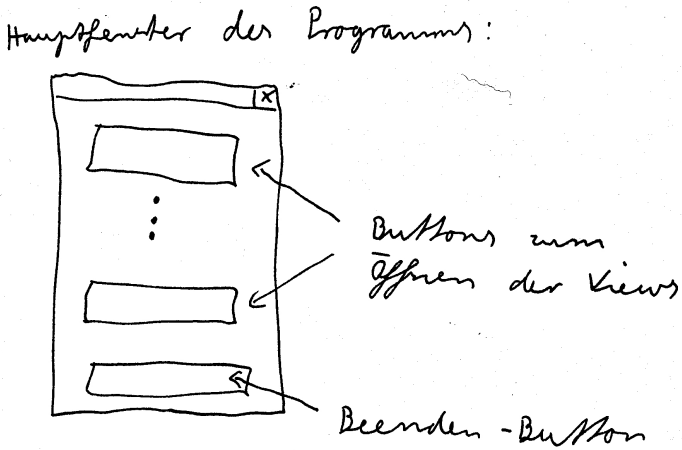
\includegraphics[width=14cm]{mainwindow.png}
\end{center}

\section{Die Tabellenansicht}

\begin{center}
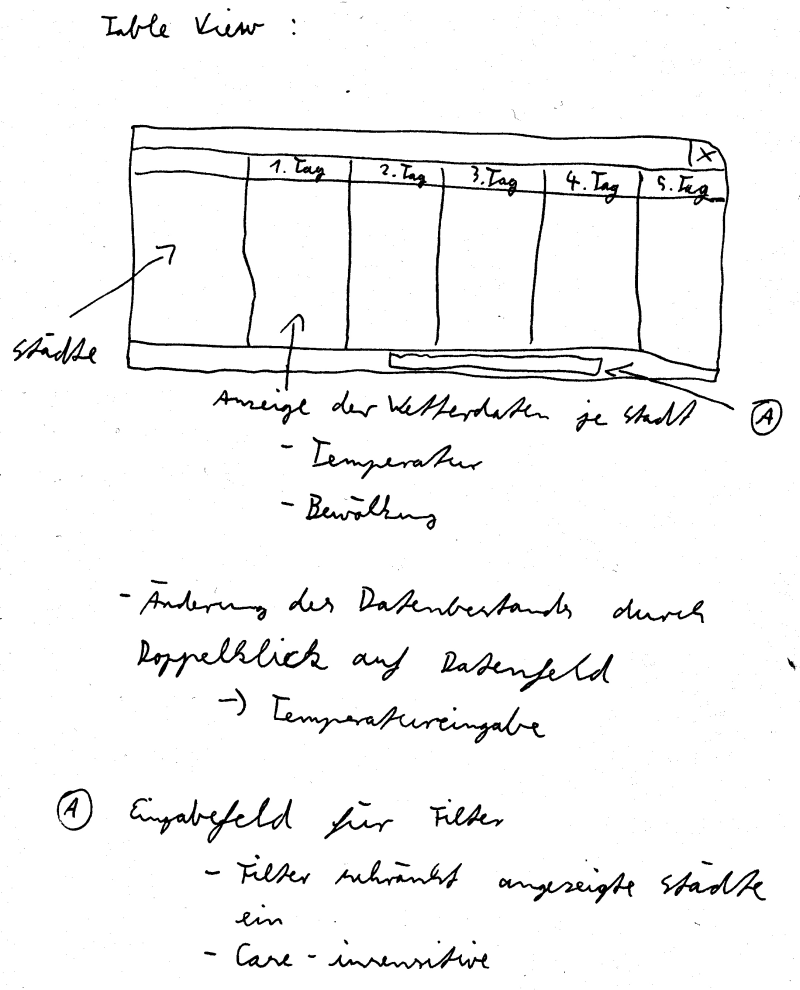
\includegraphics[width=14cm]{table_view.png}
\end{center}

\section{Die Ortsansicht}

\begin{center}
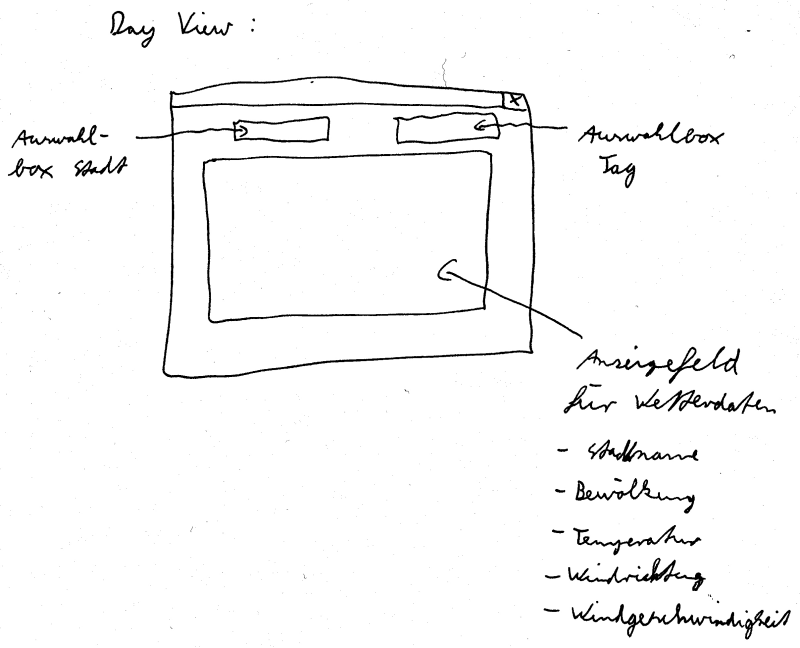
\includegraphics[width=14cm]{day_view.png}
\end{center}

\section{Die Temperaturansicht}

\begin{center}
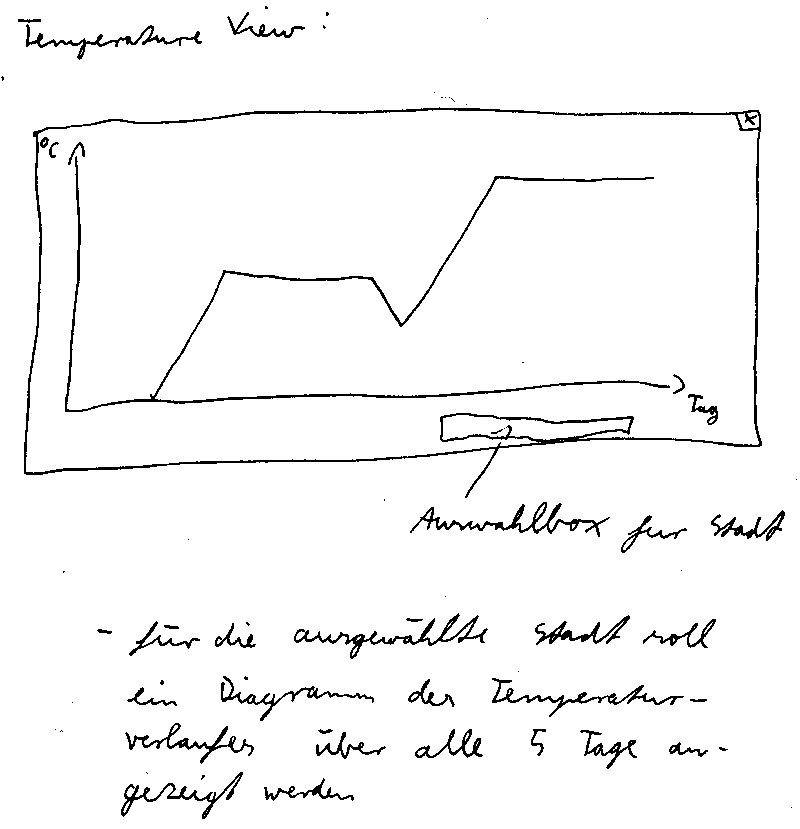
\includegraphics[width=14cm]{temperature_view.png}
\end{center}

\section{Die Weltansicht}

\begin{center}
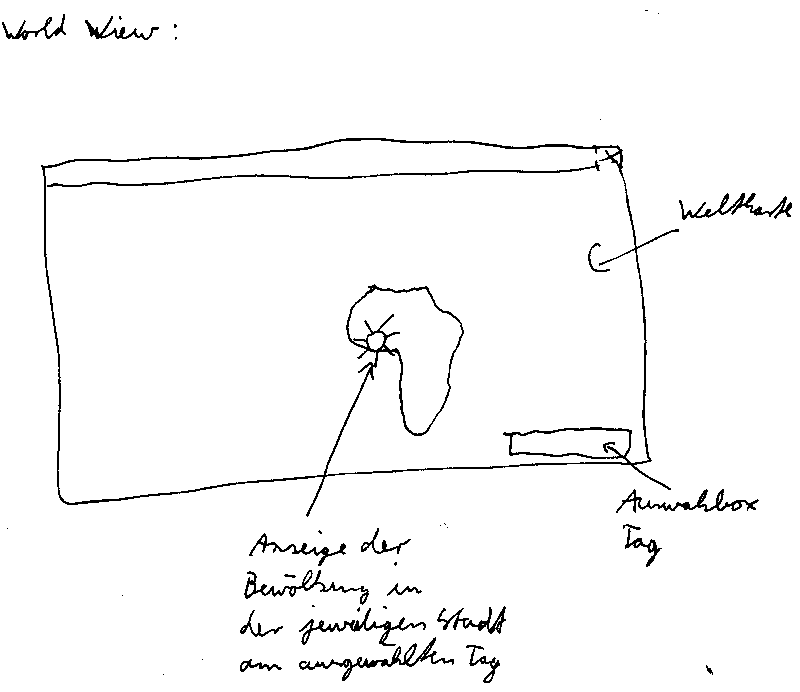
\includegraphics[width=14cm]{world_view.png}
\end{center}

\end{document}


\sectionframe{Entwurf und Entwicklung}

\begin{frame}
    \frametitle{Allgemeines zum Entwurf}
    \begin{itemize}
        \item Ausgehend von Analyse
        \item Kleines Projekt
        \item Keine "Kundenw\"unsche"
    \end{itemize}
\end{frame}
\begin{frame}
    \frametitle{Grobentwurf}
    \begin{itemize}
        \item Grobentwurf durch MVC impliziert
        \item Unterteilung in
        \begin{itemize}
          \item Views
          \item Model
          \item Storage
        \end{itemize}
        \item 3-Schichten-Architektur
    \end{itemize}
\end{frame}
\begin{frame}
    \frametitle{Grobentwurf}
    \begin{center}
        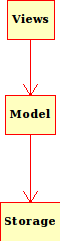
\includegraphics[width=1cm]{../design/grobentwurf.png}
    \end{center}
\end{frame}
\begin{frame}
    \frametitle{Feinentwurf}
    \begin{itemize}
        \item Verfeinerung des Views-Moduls
        \item Definition der Model-Eigenschaften
        \item Festlegung der Strukturen zum Datenaustausch
        \item Definition des Storage-Interfaces
    \end{itemize}
\end{frame}
\begin{frame}
    \frametitle{Feinentwurf}
    \begin{center}
        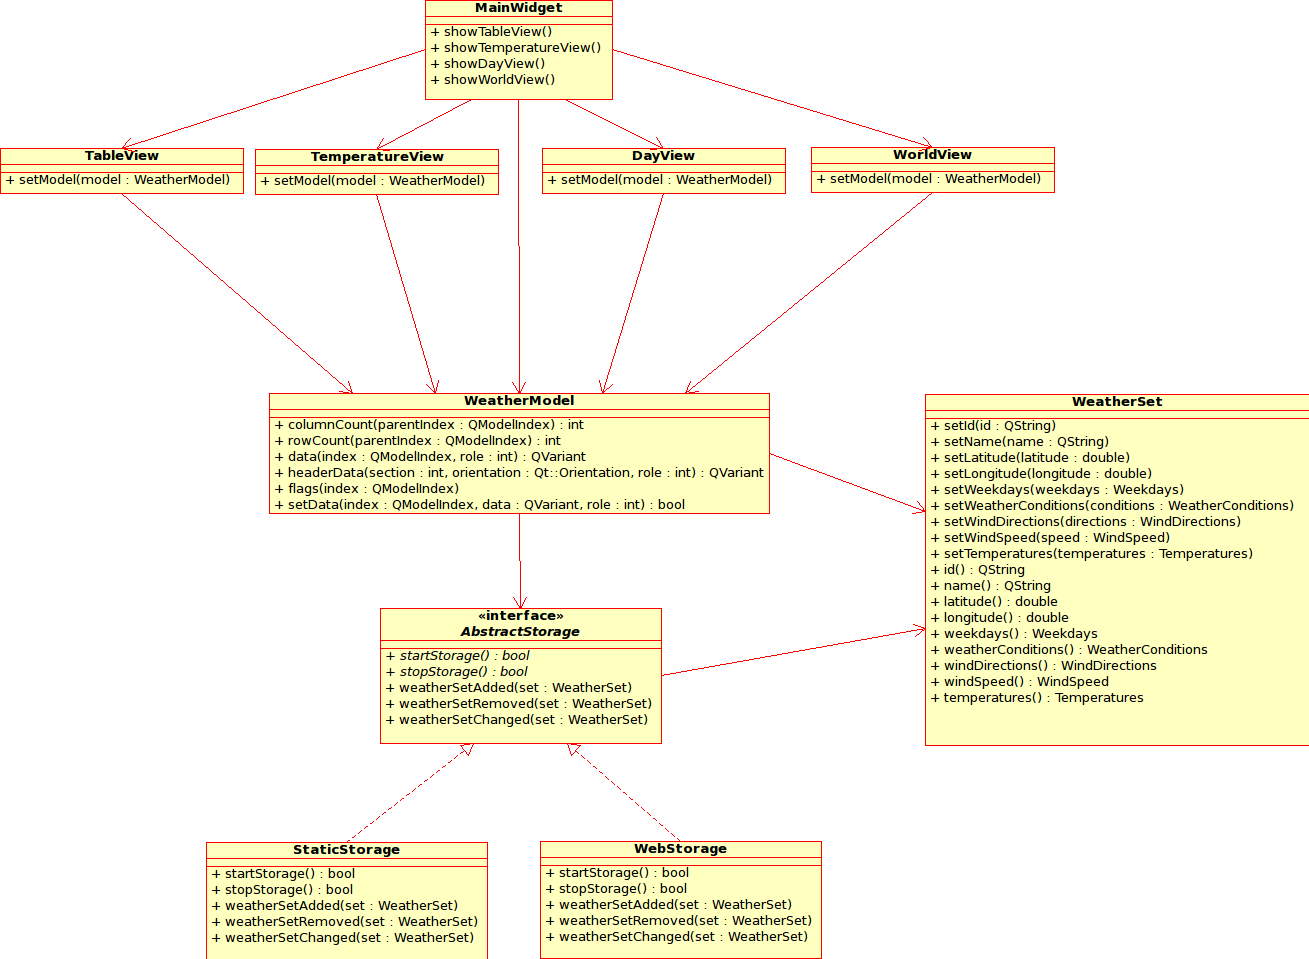
\includegraphics[width=10cm]{../design/feinentwurf.png}
    \end{center}
\end{frame}
\begin{frame}
    \frametitle{Allgemeines zur Entwicklung}
    \begin{itemize}
        \item Basiert auf C++/Qt
        \begin{itemize}
          \item Entwicklung unter Linux
          \item Produkt lauff\"ahig unter MS Windows
        \end{itemize}
        \item Nutzung des MVC-Frameworks von Qt
    \end{itemize}
\end{frame}

% \begin{frame}[fragile]
%     \frametitle{Beispiel: Proxy Model}
% \begin{tiny}
% \begin{verbatim}
% class LocationFilterProxy : public QSortFilterProxyModel
% {
%   Q_OBJECT
%   public:
%     LocationFilterProxy(QObject *parent)
%       : QSortFilterProxyModel(parent) {}
%
%   public Q_SLOTS:
%     void setLocationName(const QString &locationName)
%     {
%       mLocationName = locationName;
%       invalidateFilter();
%     }
%
%   protected:
%     virtual bool filterAcceptsRow(int row, const QModelIndex&) const
%     {
%       if (mLocationName.isEmpty())
%         return true;
%
%       const QModelIndex index = sourceModel()->index(row, 0);
%       const QString location = index.data(WeatherModel::NameRole).toString();
%
%       return location.toLower().contains(mLineEdit->text().toLower());
%     }
%
%   private:
%     QString *mLocationName;
% };
% \end{verbatim}
% \end{tiny}
% \end{frame}

\begin{frame}
    \frametitle{Demo}
    \begin{center}
        \large{Programmvorf\"uhrung}
    \end{center}
\end{frame}


\end{document}
